% Beamer presentation
\documentclass[11pt,aspectratio=43,ignorenonframetext,t]{beamer}

% Presentation settings
\mode<presentation>{
  \usetheme[framenumber,titleframestart=1]{UoM_alex}
  \usefonttheme{professionalfonts} % using non standard fonts for beamer
  \usefonttheme{serif}
  \usepackage{fontspec}
  \setmainfont[Ligatures=TeX]{Arial}
}

% Handout settings
\mode<article>{
  \usepackage{fullpage}
  \usepackage{fontspec}
  \setmainfont[Ligatures=TeX]{Arial}
  \setlength{\parskip}{1.5\baselineskip} % correct beamer line spacings
  \setlength{\parindent}{0cm}
  \usepackage{enumitem}
  \setlist[itemize]{topsep=0pt}
}

 % Packages
\usepackage{graphicx}
\graphicspath{{./images/png}} % generic graphics path; overridden if necessary
\usepackage{amsmath}
\allowdisplaybreaks[1] % allow eqnarrays to break across pages
\usepackage{amssymb} 
\usepackage[HTML]{xcolor}
\definecolor{uomlinkblue}{HTML}{0071BC}
\usepackage{hyperref}
\hypersetup{
  colorlinks=true,
  linkcolor=uomlinkblue,
  filecolor=uomlinkblue,      
  urlcolor=uomlinkblue,
  pdflang={en-GB},
}
\usepackage[document]{ragged2e} % left aligned text for accessibility
\usepackage{tikz}
\usetikzlibrary{positioning, arrows, arrows.meta}
\usepackage{unicode-math} % unicode maths for accessibility
\usepackage{pdfcomment}   % for alt text for accessibility
\usepackage{rotating}     % allow portrait figures and tables
\usepackage{subfigure}    % allow matrices of figures
\usepackage{float}        % allows H option on floats to force here placement
\usepackage{multirow}     % allows merging of rows in tables
\usepackage{tabularx}     % allows fixed width tables
\usepackage{ctable}       % modifies \hline for use in table
\usepackage{bm}           % allow bold fonts in equations
\usepackage{pgf}          % allow graphics manipulation
\usepackage{etoolbox}
  
% Custom commands
\newcolumntype{Z}{>{\centering\arraybackslash}X}  % tabularx centered columns 

\makeatletter
  \DeclareRobustCommand{\em}
  {
    \@nomath\em
    \if b
      \expandafter\@car\f@series\@nil \normalfont
    \else
      \bfseries
    \fi
  }
\makeatother

\makeatletter
  \preto{\@verbatim}{\topsep=0pt \partopsep=0pt}
\makeatother

\def\checkmark{
  \tikz\fill[scale=0.4](0,.35) -- (.25,0) -- (1,.7) -- (.25,.15) -- cycle;
}

% Counters
\newcounter{example_number} % keep track of the example questions

% Frontmatter
\newcommand{\cmclecture}[1]{
  \title{Combinatorial Mesh Calculus (CMC): Lecture #1}
}
\author{
  Lectured by:
  \href{https://scholar.google.com/citations?user=x4R-snQAAAAJ&hl=en}
  {Dr. Kiprian Berbatov}$^1$\\
  \smallskip
  Lecture Notes Compiled by:
  \href{https://scholar.google.com/citations?user=CoIpITkAAAAJ&hl=en}
  {Muhammad Azeem}$^1$\\
  \smallskip
  Under the supervision of:
  \href{https://scholar.google.co.uk/citations?user=3nWJe5wAAAAJ&hl=en}
  {Prof. Andrey P. Jivkov}$^1$\\
  \smallskip
  {\tiny $^1$Department of Mechanical and Aerospace Engineering,
    The University of Manchester, Oxford Road, Manchester M13 9PL, UK}
}

% Special frames
\newcommand{\cmctitleframe}{
  \titlepage
  \begin{tikzpicture}[remember picture,overlay]
    \node[anchor=south east] at (current page.south east) {
      \href{https://youtube.com/@kipi.berbatov}{
        
\includegraphics[width=1.5cm]{youtube-icon.png}
      }
    };
  \end{tikzpicture}
}
\newcommand{\cmcendframe}{
  \begin{figure}
    \centering
    
\includegraphics[width=0.85\linewidth]{Thanks.png}
  \end{figure}
}

\cmclecture{110}
\date{29 October 2025}

\begin{document}

%========================= TITLE =========================
\begin{frame}
  \cmctitleframe
\end{frame}


\begin{frame}{Coordinate Patch in Polar Form}
\vspace{-0.2cm}
\begin{block}{Example - Setting}
Let \(U=(\tfrac12,1]\times(-\tfrac{\pi}{6},\tfrac{\pi}{6})\) and define
\vspace{-0.2cm}
\[
f:U\to\mathbb{R}^2,\qquad f(r,\phi)=(r\cos\phi,\,r\sin\phi).
\]
Then the image
\vspace{-0.3cm}
\[
V=\operatorname{Im}f=\{(r\cos\phi,\,r\sin\phi)\mid r\in(\tfrac12,1],\,\phi\in(-\tfrac{\pi}{6},\tfrac{\pi}{6})\}
\]
is an annular sector in \(\mathbb{R}^2\).
\end{block}
\vspace{-0.5cm}
\begin{center}
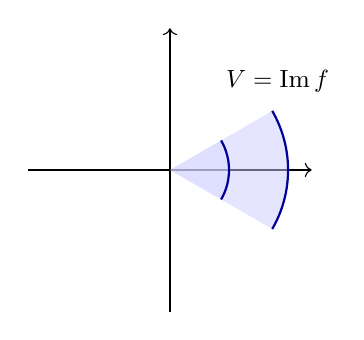
\begin{tikzpicture}[scale=1.5]
% axes
\draw[->] (-1.2,0)--(1.2,0);
\draw[->] (0,-1.2)--(0,1.2);
% annular sector
\fill[blue!10, opacity=0.5] (0,0) -- (30:0.5) arc (30:-30:0.5) -- cycle;
\fill[blue!20, opacity=0.5] (0,0) -- (30:1) arc (30:-30:1) -- cycle;
\draw[thick,blue!60!black] (30:0.5) arc (30:-30:0.5);
\draw[thick,blue!60!black] (30:1) arc (30:-30:1);
\node at (0.9,0.75) {\small $V=\mathrm{Im}\,f$};
\end{tikzpicture}
\end{center}
\end{frame}


\begin{frame}{Exterior Derivative in \(\mathbb{R}^3\)}
\begin{block}{Definition}
For a smooth manifold \(M=\mathbb{R}^3\), the exterior derivative (ED)
\[
d_p:\Omega^pM\to\Omega^{p+1}M
\]
satisfies \(d_{p+1}\circ d_p=0\) and the graded Leibniz rule.
\end{block}

\begin{block}{Concrete Computations}
Let \(f:\mathbb{R}^3\to\mathbb{R}\).
\[
d_0f=\frac{\partial f}{\partial x}dx+\frac{\partial f}{\partial y}dy+\frac{\partial f}{\partial z}dz.
\]
For a \(1\)-form \(\omega=f_xdx+f_ydy+f_zdz\),
\end{block}
\end{frame}

\begin{frame}{Example}
\begin{block}{Concrete Computations}
\[
\begin{aligned}
d_1\omega
&=d(f_x)\wedge dx+d(f_y)\wedge dy+d(f_z)\wedge dz\\[3pt]
&=(f_{zy}-f_{yz})\,dy\wedge dz+(f_{xz}-f_{zx})\,dz\wedge dx+(f_{yx}-f_{xy})\,dx\wedge dy.
\end{aligned}
\]
Thus \(d_1\omega\) corresponds to \(\operatorname{curl}(f_x,f_y,f_z)\).
\end{block}

\begin{block}{For a \(2\)-form}
If \(\eta=f_x\,dy\wedge dz+f_y\,dz\wedge dx+f_z\,dx\wedge dy\), then
\[
d_2\eta=(f_{x,x}+f_{y,y}+f_{z,z})\,dx\wedge dy\wedge dz,
\]
which represents the divergence \(\nabla\!\cdot\!(f_x,f_y,f_z)\).
\end{block}
\end{frame}


\begin{frame}{Differential Operators as ED}
\begin{block}{In \(\mathbb{R}^2\)}
\[
\begin{aligned}
&d_0f = \nabla f=(f_x,f_y),\\[3pt]
&d_1(f_xdx+f_ydy) = (f_{yx}-f_{xy})dx\wedge dy \Rightarrow \text{scalar curl},\\[3pt]
&d_1\circ d_0=0\ \Rightarrow\ \operatorname{curl}(\nabla f)=0.
\end{aligned}
\]
\end{block}
\begin{center}
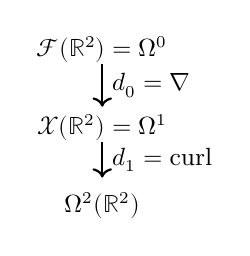
\begin{tikzpicture}[scale=0.9]
\node at (0,1.3) {\small $\mathcal{F}(\mathbb{R}^2)=\Omega^0$};
\node at (0,0.2) {\small $\mathcal{X}(\mathbb{R}^2)=\Omega^1$};
\node at (0,-0.9) {\small $\Omega^2(\mathbb{R}^2)$};
\draw[->, thick] (0,1.1)--(0,0.5) node[midway,right]{\small $d_0=\nabla$};
\draw[->, thick] (0,0)--(0,-0.5) node[midway,right]{\small $d_1=\operatorname{curl}$};
\end{tikzpicture}
\end{center}
\end{frame}

\begin{frame}{Differential Operators as ED}
    \begin{block}{In \(\mathbb{R}^3\)}
\[
\begin{aligned}
&d_0f = \nabla f,\\[3pt]
&d_1(f_xdx+f_ydy+f_zdz)=\operatorname{curl}(f_x,f_y,f_z),\\[3pt]
&d_2(f_xdy\wedge dz+\dots)=\operatorname{div}(f_x,f_y,f_z),\\[3pt]
&d_2\circ d_1=0\ \Rightarrow\ \nabla\cdot(\nabla\times A)=0.
\end{aligned}
\]
\end{block}
\begin{center}
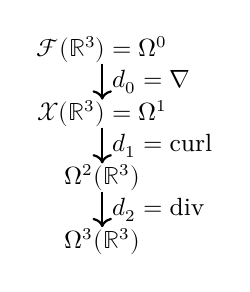
\begin{tikzpicture}[scale=0.9]
\node at (0,1.3) {\small $\mathcal{F}(\mathbb{R}^3)=\Omega^0$};
\node at (0,0.4) {\small $\mathcal{X}(\mathbb{R}^3)=\Omega^1$};
\node at (0,-0.5) {\small $\Omega^2(\mathbb{R}^3)$};
\node at (0,-1.4) {\small $\Omega^3(\mathbb{R}^3)$};
\draw[->, thick] (0,1.1)--(0,0.6) node[midway,right]{\small $d_0=\nabla$};
\draw[->, thick] (0,0.2)--(0,-0.3) node[midway,right]{\small $d_1=\operatorname{curl}$};
\draw[->, thick] (0,-0.7)--(0,-1.2) node[midway,right]{\small $d_2=\operatorname{div}$};
\end{tikzpicture}
\end{center}
\end{frame}

\begin{frame}{Pullback of Differential Forms}
\begin{block}{Definition}
Let \(M,N\) be smooth manifolds and \(f\in C^\infty(M,N)\).
For a \(1\)-form \(\omega\in\Omega^1N\) with local expression
\[
\omega = h_1\,dy_1+\cdots+h_n\,dy_n,\quad h_i\in\mathcal{F}(N),
\]
the pullback \(f^*\omega\in\Omega^1M\) is defined by
\[
f^*\omega=(h_1\circ f)\,d(y_1\circ f)+\cdots+(h_n\circ f)\,d(y_n\circ f).
\]
It extends naturally to exterior powers: \(f^*(\omega\wedge\eta)=f^*\omega\wedge f^*\eta.\)
\end{block}
\end{frame}

\begin{frame}{Pullback of Differential Forms}
    \begin{block}{Example}
Let \(M=N=\mathbb{R}^2\), \(f(r,\phi)=(r\cos\phi,r\sin\phi)\), and \(\omega=-y\,dx+x\,dy\). Then
\[
\begin{aligned}
f^*\omega =& -(r\sin\phi)\,d(r\cos\phi)+(r\cos\phi)\,d(r\sin\phi)\\[3pt]
=& -(r\sin\phi)(\cos\phi\,dr-r\sin\phi\,d\phi)\\
&+(r\cos\phi)(\sin\phi\,dr+r\cos\phi\,d\phi)\\[3pt]
=&r^2\,d\phi.
\end{aligned}
\]
\end{block}
\end{frame}


\begin{frame}{Compatibility of Pullback and ED}
\vspace{-0.3cm}
\begin{block}{Theorem (Compatibility of Pullback and Exterior Derivative)}
Let \(M,N\) be smooth manifolds and \(f\in C^\infty(M,N)\) a smooth map. For each degree \(p\in\mathbb{N}\), the pullback operator
\vspace{-0.2cm}
\[
f_p^*:\Omega^p(N)\to\Omega^p(M)
\]
\vspace{-0.1cm}
commutes with the exterior derivative, i.e.
\vspace{-0.2cm}
\[
d_p^M\circ f_p^* = f_{p+1}^*\circ d_p^N.
\]
\vspace{-0.1cm}
In other words, taking the pullback of a form and then differentiating gives the same result as differentiating first and then taking the pullback:
\vspace{-0.2cm}
\[
f^*(d\omega)=d(f^*\omega), \quad \forall\,\omega\in\Omega^p(N).
\]
This shows that the exterior derivative is a \emph{natural operator} with respect to smooth maps between manifolds.
\end{block}

\end{frame}

\begin{frame}{Example}
\vspace{-0.2cm}
    \begin{center}
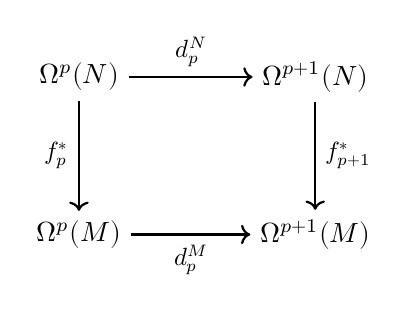
\begin{tikzpicture}[scale=1.0]
\node (A1) at (0,1.2) {$\Omega^p(N)$};
\node (A2) at (3,1.2) {$\Omega^{p+1}(N)$};
\node (B1) at (0,-0.8) {$\Omega^p(M)$};
\node (B2) at (3,-0.8) {$\Omega^{p+1}(M)$};
\draw[->, thick] (A1)--(A2) node[midway,above]{\small $d_p^N$};
\draw[->, thick] (A1)--(B1) node[midway,left]{\small $f_p^*$};
\draw[->, thick] (B1)--(B2) node[midway,below]{\small $d_p^M$};
\draw[->, thick] (A2)--(B2) node[midway,right]{\small $f_{p+1}^*$};
\end{tikzpicture}
\end{center}
\vspace{-0.3cm}
\begin{block}{Example}
Let \(M=N=\mathbb{R}^2\), \(f(r,\phi)=(r\cos\phi,r\sin\phi)\), \(\omega=dx\wedge dy\):
\[
\begin{aligned}
f^*dx &= \cos\phi\,dr - r\sin\phi\,d\phi,\\
f^*dy &= \sin\phi\,dr + r\cos\phi\,d\phi,\\
f^*(dx\wedge dy)&=(f^*dx)\wedge(f^*dy)=r\,dr\wedge d\phi.
\end{aligned}
\]
\vspace{-0.1cm}
\end{block}
\end{frame}

\begin{frame}{Trace of Differential Forms on Submanifolds}
\begin{block}{Definition}
Let \(M\) be a smooth manifold and \(N\subseteq M\) a submanifold with inclusion map
\[
\iota_N:N\hookrightarrow M,\quad \iota_N(x)=x.
\]
The \textbf{trace} (restriction) of forms is the pullback
\[
\operatorname{tr}_N=\iota_N^*:\Omega^\bullet M\to\Omega^\bullet N.
\]
If \(N\subseteq\partial M\), this represents the restriction of forms to the boundary.
\end{block}
\end{frame}


\begin{frame}{Example}
\vspace{-0.3cm}
\begin{block}{Example}
Let \(M=\mathbb{R}^2\), \(N=S^1\subseteq M\), and \(\omega=x\,dy - y\,dx\).
The inclusion \(\iota_{S^1}:S^1\to\mathbb{R}^2\) gives
\vspace{-0.3cm}
\begin{align*}
\operatorname{tr}_{S^1}\omega
=&(x\,dy - y\,dx)\big|_{S^1}\\
=&(r\cos\phi)(r\cos\phi\,d\phi)-(r\sin\phi)(-r\sin\phi\,d\phi) =r^2d\phi,
\end{align*}
\[
\text{and for \(r=1\),\ }\operatorname{tr}_{S^1}\omega=d\phi.
\]
\end{block}
\vspace{-0.3cm}
\begin{center}
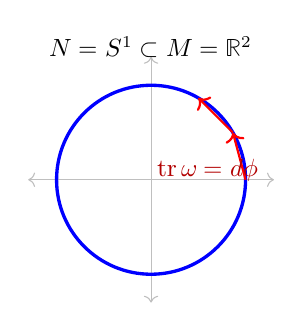
\begin{tikzpicture}[scale=1.2]
% plane arrows
\foreach \a in {0,90,180,270}{
\draw[->,gray!50] (0,0)--({1.3*cos(\a)},{1.3*sin(\a)});
}
% circle
\draw[very thick,blue] (0,0) circle (1);
\node at (0,1.4) {\small $N=S^1\subset M=\mathbb{R}^2$};
\draw[->, thick, red] (1,0)--(0.866,0.5);
\draw[->, thick, red] (0.866,0.5)--(0.5,0.866);
\node[red!70!black] at (0.6,0.1) {\small $\operatorname{tr}\omega=d\phi$};
\end{tikzpicture}
\end{center}
\end{frame}


\begin{frame}{Orientation of Smooth Manifolds}
\vspace{-0.1cm}
\begin{block}{Definition}
Let \(M\) be a smooth manifold of dimension \(D\).
Since the space of top–degree forms \(\Omega^D M\) is locally $1$–dimensional, every element \(\omega\in\Omega^D M\) can be written locally as
\vspace{-0.2cm}
\[
\omega=f\,dx_1\wedge dx_2\wedge\cdots\wedge dx_D,\qquad f\in\mathcal{F}(M).
\]
If \(f(x)\neq 0\) for all \(x\in M\), then \(\omega\) is said to be a \textbf{nonvanishing $D$–form}, and \(M\) is called \textbf{orientable}.
A choice of such an $\omega$ (and identifying all positive scalar multiples of $\omega$ as equivalent) defines an \textbf{orientation} of \(M\).

If \(M\) is connected and orientable, it admits exactly two possible orientations, represented by \(\omega\) and \(-\omega\).
If \(M\) is disconnected, each connected component may be oriented independently.

\end{block}

\end{frame}

\begin{frame}{Orientation of Smooth Manifolds}
Intuitively, an orientation distinguishes between the two possible “directions of measurement” on \(M\): one associated with $\omega$ (positive orientation) and the other with $-\omega$ (negative orientation).
\begin{block}{Example}
\(\mathbb{R}^D\) is orientable with orientation
\[
\omega=dx_1\wedge dx_2\wedge\cdots\wedge dx_D,
\quad \text{or its opposite } -dx_1\wedge\cdots\wedge dx_D.
\]
\end{block}

\begin{center}
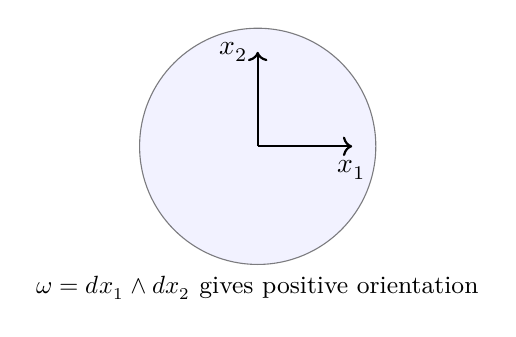
\begin{tikzpicture}[scale=1.0]
\draw[fill=blue!10,opacity=0.5] (0,0) circle (1.5);
\draw[->,thick] (0,0)--(1.2,0);
\draw[->,thick] (0,0)--(0,1.2);
\node at (1.2,-0.3) {$x_1$};
\node at (-0.3,1.2) {$x_2$};
\node at (0,-1.8) {\small $\omega=dx_1\wedge dx_2$ gives positive orientation};
\end{tikzpicture}
\end{center}
\end{frame}

\begin{frame}{Outward-Pointing Vector Fields}
\begin{block}{Definition}
Let \(M\subseteq\mathbb{R}^D\) be a $D$–dimensional manifold with boundary.
A vector field \(X\in\mathcal{X}(M)\) is called \textbf{outward-pointing} on $\partial M$
if near every boundary point it locally points outside $M$.
\end{block}

\begin{block}{Examples}
\begin{itemize}
\item \(M=\overline{B}_1(0,0)\subseteq\mathbb{R}^2,\quad X=x\frac{\partial}{\partial x}+y\frac{\partial}{\partial y}\);
\item \(M=\overline{B}_1(0,0,0)\subseteq\mathbb{R}^3,\quad X=x\frac{\partial}{\partial x}+y\frac{\partial}{\partial y}+z\frac{\partial}{\partial z}\).
\end{itemize}
\end{block}

\begin{center}
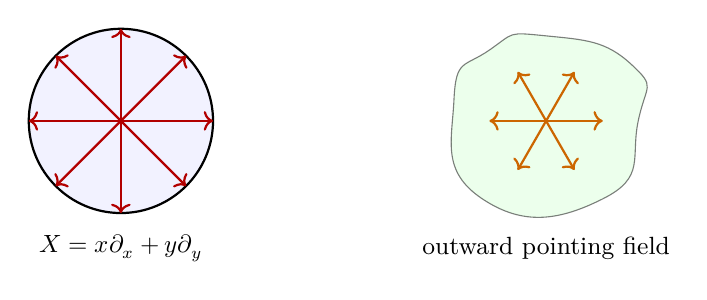
\begin{tikzpicture}[scale=0.9]
% --- 2D ball ---
\begin{scope}[xshift=-3cm]
\fill[blue!10,opacity=0.5] (0,0) circle (1.3);
\draw[thick] (0,0) circle (1.3);
\foreach \a in {0,45,90,135,180,225,270,315}{
\draw[->,red!70!black,thick] (0,0)--({1.3*cos(\a)},{1.3*sin(\a)});
}
\node at (0,-1.8) {\small $X=x\partial_x+y\partial_y$};
\end{scope}

% --- 3D "potato" sketch ---
\begin{scope}[xshift=3cm]
\draw[fill=green!15,opacity=0.5] plot[smooth cycle,tension=1] coordinates{(0,1.2) (1.2,0.8) (1.3,0) (0.8,-1.1) (-0.9,-1.1) (-1.3,0.3) (-0.8,1)};
\foreach \a in {0,60,120,180,240,300}{
\draw[->,orange!80!black,thick] (0,0)--({0.8*cos(\a)},{0.8*sin(\a)});
}
\node at (0,-1.8) {\small outward pointing field};
\end{scope}
\end{tikzpicture}
\end{center}
\end{frame}


\begin{frame}{The Induced Orientation on Boundaries}
\begin{block}{Theorem (Induced Orientation)}
Let \(M\) be an orientable $D$–manifold with boundary \(S=\partial M\)
and orientation form \(\omega\in\Omega^D M\).
If \(X\in\mathcal{X}(M)\) is outward-pointing, then
\[
\omega_S = \operatorname{tr}_{\partial M}\!\bigl(\iota_X\omega\bigr)\in\Omega^{D-1}(S)
\]
defines an orientation form on \(S\), called the \textbf{induced orientation}.
\end{block}

\end{frame}

\begin{frame}{Example}
\vspace{-0.2cm}
    \begin{block}{Example 1: Half–Plane}
Let \(M=[0,\infty)\times\mathbb{R}\), \(S=\{0\}\times\mathbb{R}\),
\vspace{-0.2cm}
\[
X=-\frac{\partial}{\partial x},\quad \omega=dx\wedge dy.
\]
Then
\vspace{-0.2cm}
\[
\iota_X(dx\wedge dy)
=\iota_{-\partial_x}(dx\wedge dy)
=-\,\iota_{\partial_x}(dx\wedge dy)
=-\,dy.
\]
Thus \(\omega_S=-dy\): the boundary inherits the leftward orientation.
\end{block}

\begin{center}
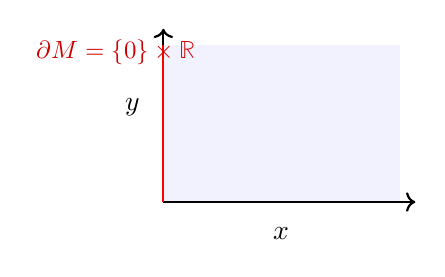
\begin{tikzpicture}[scale=1.0]
\fill[blue!10,opacity=0.5] (0,0) rectangle (3,2);
\draw[->,thick] (0,0)--(3.2,0);
\draw[->,thick] (0,0)--(0,2.2);
\node at (1.5,-0.4) {$x$}; \node at (-0.4,1.2) {$y$};
\draw[thick,red] (0,0)--(0,2);
\node[red!80!black] at (-0.6,1.9) {\small $\partial M=\{0\}\times\mathbb{R}$};
\end{tikzpicture}
\end{center}
\end{frame}

\begin{frame}{Induced Orientation in 2D and 3D Balls}
\vspace{-0.2cm}
\begin{block}{Example 2: Disk in \(\mathbb{R}^2\)}
\vspace{-0.7cm}
\[
\text{\(M=B_1(0,0)\), \(\partial M=S^1\),\ \ }X=x\partial_x+y\partial_y,\qquad \omega_M=dx\wedge dy.
\]
\vspace{-0.4cm}
\[
\text{Then\ \ }\iota_X\omega_M = \iota_{x\partial_x+y\partial_y}(dx\wedge dy)
= x\,dy - y\,dx.
\]
In polar coordinates \(x=r\cos\phi,\ y=r\sin\phi\), so
\vspace{-0.2cm}
\[
x\,dy - y\,dx = r^2\,d\phi \quad \Rightarrow \quad
\operatorname{tr}_{S^1}(\iota_X\omega_M)=d\phi.
\]
Hence, \(S^1\) inherits counterclockwise orientation.
\end{block}
\vspace{-0.2cm}
\begin{center}
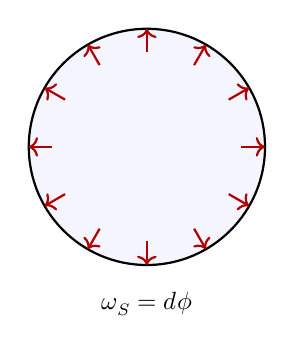
\begin{tikzpicture}[scale=1.0]
\fill[blue!10,opacity=0.4] (0,0) circle (1.5);
\draw[thick] (0,0) circle (1.5);
\foreach \a in {0,30,...,330}{
\draw[->,red!70!black,thick] ({1.2*cos(\a)},{1.2*sin(\a)}) -- ({1.5*cos(\a)},{1.5*sin(\a)});
}
\node at (0,-2) {\small $\omega_S=d\phi$};
\end{tikzpicture}
\end{center}
\end{frame}


\begin{frame}{3D Ball: Induced Orientation on the Sphere}
\begin{block}{Example 3: Ball in \(\mathbb{R}^3\)}
\(M=B_1(0,0,0)\), \(\partial M=S^2\),
\[
X=x\partial_x+y\partial_y+z\partial_z,\qquad
\omega_M=dx\wedge dy\wedge dz.
\]
Then
\[
\iota_X\omega_M
= x\,dy\wedge dz + y\,dz\wedge dx + z\,dx\wedge dy.
\]
In spherical coordinates \(x=r\sin\theta\cos\phi,\ y=r\sin\theta\sin\phi,\ z=r\cos\theta\),
we have
\[
\operatorname{tr}_{S^2}(\iota_X\omega_M)
= r^2\sin\theta\,d\theta\wedge d\phi.
\]
This $2$–form defines the standard orientation of $S^2$.
\end{block}
\end{frame}

\begin{frame}{Visualization}
    \begin{center}
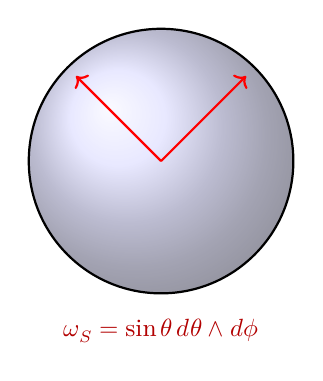
\begin{tikzpicture}[scale=1.2]
\shade[ball color=blue!20,opacity=0.6] (0,0) circle (1.4);
\draw[thick] (0,0) circle (1.4);
\draw[->,thick,red] (0,0)--(0.9,0.9);
\draw[->,thick,red] (0,0)--(-0.9,0.9);
\node[red!70!black] at (0,-1.8) {\small $\omega_S=\sin\theta\,d\theta\wedge d\phi$};
\end{tikzpicture}
\end{center}
\end{frame}


\begin{frame}{Spherical Coordinates}
\begin{block}{Spherical chart on \(S^2\) (radius \(1\))}
Standard spherical coordinates
\vspace{-0.2cm}
\[
x=\sin\theta\cos\phi,\quad
y=\sin\theta\sin\phi,\quad
z=\cos\theta, \theta\in(0,\pi),\ \phi\in(0,2\pi)
\]
yield the induced orientation $2$–form
\vspace{-0.2cm}
\[
\omega_{S^2}=\sin\theta\,d\theta\wedge d\phi.
\]
Here \(d\theta\wedge d\phi\) is ordered so that \((\partial_\theta,\partial_\phi)\) agrees with the outward normal orientation.
\(\sin\theta\) is the Jacobian density (area scale factor) of the chart; it vanishes only at the poles \(\theta=0,\pi\), where this chart is \emph{singular} (coordinate singularity, not a geometric one).
\end{block}

\end{frame}

\begin{frame}{Visualization}
    \begin{center}
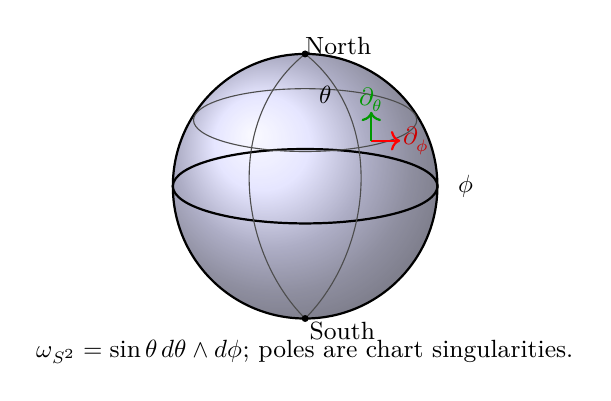
\begin{tikzpicture}[scale=1.05]
% sphere
\shade[ball color=blue!18,opacity=0.75] (0,0) circle (1.6);
\draw[thick] (0,0) circle (1.6);
% equator and latitude
\draw[thick,black] (0,0) ellipse (1.6 and 0.45); % equator
\draw[black!70] (0,0.8) ellipse (1.35 and 0.38);  % latitude (theta fixed)
% meridian (phi fixed)
\draw[black!70] (0,-1.6) .. controls (0.8,-0.8) and (1,0.8) .. (0,1.6);
\draw[black!70] (0,-1.6) .. controls (-0.8,-0.8) and (-1,0.8) .. (0,1.6);
% labels for angles
\node at (1.95,0) {\small $\phi$};
\node at (0.25,1.1) {\small $\theta$};
% small arrows for basis directions on a latitude point
\draw[->,red,thick] (0.8,0.55) -- (1.15,0.55);    % along +phi
\draw[->,green!60!black,thick] (0.8,0.55) -- (0.8,0.9); % along +theta
\node[red!80!black] at (1.35,0.55) {\small $\partial_\phi$};
\node[green!60!black] at (0.8,1.05) {\small $\partial_\theta$};
% poles
\fill (0,1.6) circle (1.2pt); \node at (0.4,1.7) {\small North};
\fill (0,-1.6) circle (1.2pt); \node at (0.45,-1.75) {\small South};
% caption
\node at (0,-2.0) {\small $\omega_{S^2}=\sin\theta\,d\theta\wedge d\phi$; poles are chart singularities.};
\end{tikzpicture}
\end{center}
\end{frame}


\begin{frame}{Curvature Intuition on \(S^2\): Meridians vs Parallels}
\begin{block}{Geodesics and geodesic curvature (unit sphere)}
\begin{itemize}
\item \textbf{Meridians} (\(\phi=\) const) and \textbf{equator} (\(\theta=\pi/2\)) are \emph{great circles} \(\Rightarrow\) geodesics with geodesic curvature \(\kappa_g=0\).
\item \textbf{Parallels} (\(\theta=\) const \(\neq\pi/2\)) are not geodesics; their geodesic curvature is \(\kappa_g=|\cos\theta|\) (nonzero away from the equator).
\item The area element (orientation form) is \(\omega_{S^2}=\sin\theta\,d\theta\wedge d\phi\): bands near the equator (\(\theta\approx \pi/2\)) have greater area density; near the poles (\(\theta\to 0,\pi\)) the density vanishes.
\end{itemize}
\end{block}

\end{frame}

\begin{frame}{Visualization}
    \begin{center}
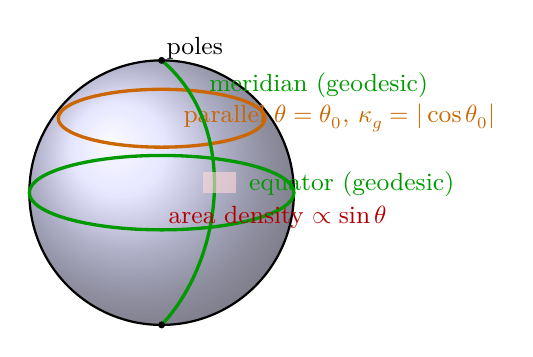
\begin{tikzpicture}[scale=1.05]
% sphere
\shade[ball color=blue!18,opacity=0.75] (0,0) circle (1.6);
\draw[thick] (0,0) circle (1.6);
% equator (geodesic)
\draw[very thick,green!60!black] (0,0) ellipse (1.6 and 0.45);
\node[green!60!black] at (2.3,0.1) {\small equator (geodesic)};
% a non-geodesic parallel
\draw[very thick,orange!80!black] (0,0.9) ellipse (1.25 and 0.35);
\node[orange!80!black] at (2.15,0.9) {\small parallel $\theta=\theta_0$, $\kappa_g=|\cos\theta_0|$};
% a meridian (geodesic)
\draw[very thick,green!60!black] (0,-1.6) .. controls (0.75,-0.8) and (0.95,0.8) .. (0,1.6);
\node[green!60!black] at (1.9,1.3) {\small meridian (geodesic)};

% small area patch to suggest density
\fill[red!15,opacity=0.6] (0.5,0) -- (0.9,0) -- (0.9,0.25) -- (0.5,0.25) -- cycle;
\node[red!70!black] at (1.4,-0.3) {\small area density $\propto \sin\theta$};

% poles
\fill (0,1.6) circle (1.2pt); \fill (0,-1.6) circle (1.2pt);
\node at (0.4,1.75) {\small poles};

\end{tikzpicture}
\end{center}

\begin{block}{Summary}
The \(\theta,\phi\) chart encodes orientation and area via \(\sin\theta\), is singular at the poles,
and separates geodesic directions (great circles) from curved parallels (nonzero \(\kappa_g\)).
\end{block}
\end{frame}

\begin{frame}{Compact Manifolds and Integration}
\begin{block}{Definition}
A manifold \(M\subseteq\mathbb{R}^D\) is \textbf{compact} if it is closed and bounded,
i.e. it lies entirely inside some finite ball \(B_R(0)\).
\end{block}

\begin{block}{Examples}
\begin{itemize}
\item Closed $D$–bricks and their boundaries,
\item Closed $D$–balls $\overline{B}_1(0)$ and spheres $S^{D-1}$.
\end{itemize}
\end{block}

\end{frame}


\begin{frame}{Integration}
\vspace{-0.2cm}
    \begin{block}{Smooth Oriented $D$–Manifolds}
For compact, oriented $M$, integration is a linear map
\vspace{-0.3cm}
\[
\int_M:\Omega^D M\to\mathbb{R}
\]
satisfying:
\begin{enumerate}
\item \textbf{Additivity:} If \(M=M_1\cup M_2\) with same orientation,
\vspace{-0.3cm}
\[
\int_M\omega = \int_{M_1}\operatorname{tr}_{M_1}\omega + \int_{M_2}\operatorname{tr}_{M_2}\omega.
\]
\item \textbf{Change of Variables:} If \(\phi:M\to N\) is an orientation–preserving diffeomorphism,
\vspace{-0.3cm}
\[
\int_N\omega=\int_M\phi^*\omega.
\]
\end{enumerate}
\end{block}
\end{frame}

\begin{frame}{Integration}
\vspace{-0.2cm}
\begin{block}{Smooth Oriented $D$–Manifolds}
\begin{enumerate}
\item[3] \textbf{Stokes–Cartan Theorem:}
\vspace{-0.3cm}
\[
\int_M d\omega=\int_{\partial M}\operatorname{tr}_{\partial M}\omega.
\]
\item[4] \textbf{Zero–Dimensional Case:}
If \(M=\{x\}\) with orientation \(\epsilon=\pm1\),
\(\displaystyle \int_{\{x\}}f=\epsilon\,f(x).\)
\end{enumerate}
\end{block}
\end{frame}


\begin{frame}{Example 1: (\(D=1\))}
\begin{block}{Statement: Newton–Leibniz Theorem}
Let \(M=[a,b]\subset\mathbb{R}\), with boundary
\(\partial M=\{a,b\}\) oriented as \(a\mapsto b\).
For \(f\in C^\infty(M)\),
\[
\omega=df=f'(x)\,dx.
\]
Then, by Stokes–Cartan:
\[
\int_{[a,b]}df
=\int_{\partial[a,b]}\operatorname{tr}f
=f(b)-f(a).
\]
\end{block}
\vspace{-0.3cm}
\begin{center}
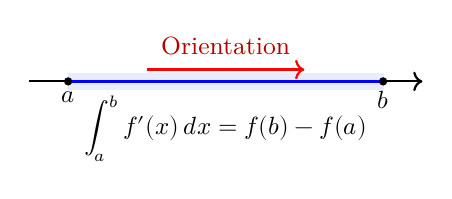
\begin{tikzpicture}[scale=1.0]
\draw[->,thick] (-0.5,0)--(4.5,0);
\filldraw[blue!20,opacity=0.4] (0,0.1) rectangle (4,-0.1);
\draw[very thick,blue] (0,0)--(4,0);
\fill (0,0) circle (1.5pt) node[below] {\small $a$};
\fill (4,0) circle (1.5pt) node[below] {\small $b$};
\draw[->,red,thick] (1,0.15)--(3,0.15);
\node[red!70!black] at (2,0.45) {\small Orientation};
\node at (2,-0.6) {\small $\displaystyle \int_a^b f'(x)\,dx=f(b)-f(a)$};
\end{tikzpicture}
\end{center}
\end{frame}


\begin{frame}{Example 2: (\(D=2\), Curve in $\mathbb{R}^2$)}
\begin{block}{Statement: Gradient Theorem }
Let $\gamma:[a,b]\to\mathbb{R}^2$ be a smooth oriented $1$–manifold with boundary $\partial\gamma=\{\gamma(a),\gamma(b)\}$,
and \(f\in C^\infty(\mathbb{R}^2)\).
The $1$–form
\[
\omega = df = \frac{\partial f}{\partial x}dx + \frac{\partial f}{\partial y}dy.
\]
Then
\[
\int_{\gamma}d f
=\int_{\partial\gamma}\operatorname{tr}_{\partial\gamma}f
=f(\gamma(b))-f(\gamma(a)).
\]
Thus, the \textbf{gradient theorem} is the $2$–dimensional instance of Stokes–Cartan.
\end{block}
\end{frame}

\begin{frame}{Visualization}
    \begin{center}
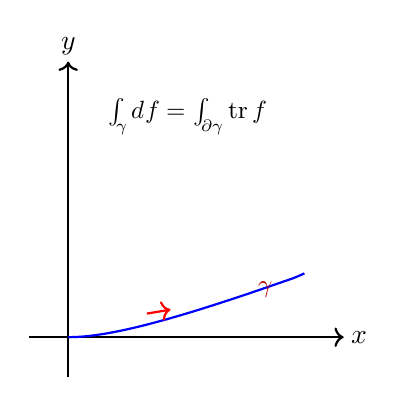
\begin{tikzpicture}[scale=1.0]
\draw[->,thick] (-0.5,0)--(3.5,0);
\draw[->,thick] (0,-0.5)--(0,3.5);
\node at (3.7,0) {$x$};
\node at (0,3.7) {$y$};
\draw[thick,blue,smooth,domain=0:3] plot(\x,{0.4*\x*\x/(1.5+\x)});
\draw[->,red,thick] (1,0.3)--(1.3,0.35);
\node[red!70!black] at (2.5,0.6) {\small $\gamma$};
\node at (1.5,2.8) {\small $\int_\gamma df=\int_{\partial\gamma}\operatorname{tr}f$};
\end{tikzpicture}
\end{center}
\end{frame}

\begin{frame}{Example 3: (\(D=2\))}
\vspace{-0.3cm}
\begin{block}{Statement: Green’s Theorem }
Let $M\subset\mathbb{R}^2$ be a compact oriented $2$–manifold with boundary $\partial M$ (positively oriented).
For a $1$–form $\omega = P\,dx + Q\,dy$,
\vspace{-0.2cm}
\[
d\omega
=\left(\frac{\partial Q}{\partial x}-\frac{\partial P}{\partial y}\right)dx\wedge dy.
\]
\vspace{-0.2cm}
Then by Stokes–Cartan,
\vspace{-0.2cm}
\[
\int_M d\omega
=\int_{\partial M}\operatorname{tr}_{\partial M}\omega.
\]
This is \textbf{Green’s theorem} in exterior–form form:
the flux of $d\omega$ across $M$ equals the trace of $\omega$ on $\partial M$.
\end{block}

\begin{center}
\vspace{-0.2cm}
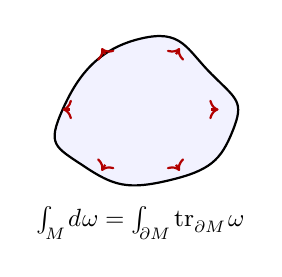
\begin{tikzpicture}[scale=0.9]
\fill[blue!10,opacity=0.5] plot[smooth cycle,tension=1] coordinates{(0,1) (1,0.5) (1.3,-0.3) (0.4,-1) (-0.8,-0.8) (-1.1,0)};
\draw[thick] plot[smooth cycle,tension=1] coordinates{(0,1) (1,0.5) (1.3,-0.3) (0.4,-1) (-0.8,-0.8) (-1.1,0)};
\foreach \a in {0,60,120,180,240,300}{
\draw[->,red!70!black,thick] ({1.0*cos(\a)},{0.9*sin(\a)})--({1.1*cos(\a)},{1.0*sin(\a)});
}
\node at (0,-1.6) {\small $\int_M d\omega=\int_{\partial M}\operatorname{tr}_{\partial M}\omega$};
\end{tikzpicture}
\end{center}
\end{frame}


\begin{frame}{Example 4: \(D=3\)}
\vspace{-0.3cm}
\begin{block}{Statement (Stokes–Cartan for a $1$–manifold in \(\mathbb{R}^3\))}
Let \(\gamma:[a,b]\to \mathbb{R}^3\) be a smooth oriented curve (a compact \(1\)–manifold \(M=\gamma([a,b])\) with
\(\partial M=\{\gamma(a),\gamma(b)\}\) and orientation from \(a\) to \(b\)).
For \(f\in \mathcal{F}(\mathbb{R}^3)=C^\infty(\mathbb{R}^3)\), the $1$–form
\vspace{-0.3cm}
\[
df=\frac{\partial f}{\partial x}\,dx+\frac{\partial f}{\partial y}\,dy+\frac{\partial f}{\partial z}\,dz.
\]
Then, by Stokes–Cartan on the \(1\)–manifold \(M\),
\vspace{-0.3cm}
\[
\boxed{\;\displaystyle \int_{\gamma} df
=\int_{\partial\gamma}\operatorname{tr}_{\partial\gamma} f
= f(\gamma(b)) - f(\gamma(a))\;}
\]
(i.e. the \emph{line integral of the exact form \(df\)} along the space curve equals the trace of \(f\) on the boundary points).
\end{block}
\end{frame}

\begin{frame}{Visualization}
    \begin{center}
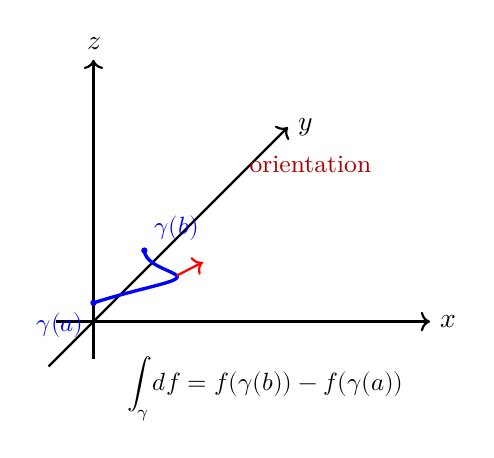
\begin{tikzpicture}[scale=0.95]
% axes
\draw[->,thick] (-0.5,0)--(4.5,0) node[right]{$x$};
\draw[->,thick] (0,-0.5)--(0,3.5) node[above]{$z$};
\draw[->,thick] (-0.6,-0.6)--(2.6,2.6) node[right]{$y$};

% space curve (projected)
\draw[very thick,blue,domain=0:3,smooth] plot ({0.4*\x+0.6*sin(80*\x)},{0.4*\x+0.25*cos(60*\x)});
% start/end
\fill[blue] ({0.4*0+0.6*sin(0)},{0.4*0+0.25*cos(0)}) circle (1.2pt) node[below left] {\small $\gamma(a)$};
\fill[blue] ({0.4*3+0.6*sin(240)},{0.4*3+0.25*cos(180)}) circle (1.2pt) node[above right] {\small $\gamma(b)$};
% orientation arrow
\draw[->,red,thick] ({0.4*1.6+0.6*sin(128)},{0.4*1.6+0.25*cos(96)}) -- ++(0.35,0.18);
\node[red!70!black] at (2.9,2.1) {\small orientation};

\node at (2.3,-0.9) {\small $\displaystyle \int_{\gamma} df=f(\gamma(b))-f(\gamma(a))$};
\end{tikzpicture}
\end{center}
\end{frame}


\begin{frame}{Example 5: (\(D=3\))}
\vspace{-0.3cm}
\begin{block}{Statement: Kelvin–Stokes Theorem }
Let \(M\subset\mathbb{R}^3\) be a smooth oriented $2$–manifold with boundary $\partial M$.
For a $1$–form \(\omega = A\,dx + B\,dy + C\,dz\),
\vspace{-0.2cm}
\[
d\omega
=\left(\frac{\partial C}{\partial y}-\frac{\partial B}{\partial z}\right)dy\wedge dz
+\left(\frac{\partial A}{\partial z}-\frac{\partial C}{\partial x}\right)dz\wedge dx
+\left(\frac{\partial B}{\partial x}-\frac{\partial A}{\partial y}\right)dx\wedge dy.
\]
Then by Stokes–Cartan:
\vspace{-0.2cm}
\[
\int_M d\omega
=\int_{\partial M}\operatorname{tr}_{\partial M}\omega.
\]
This is the \textbf{Kelvin–Stokes theorem} in exterior form notation.
\end{block}

\begin{center}
\vspace{-0.2cm}
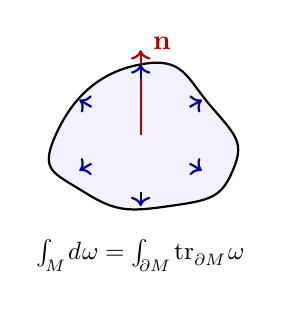
\begin{tikzpicture}[scale=0.9]
\fill[blue!10,opacity=0.5] plot[smooth cycle,tension=1] coordinates{(0,1) (1,0.4) (1.3,-0.5) (0.4,-1) (-0.8,-0.8) (-1.2,0)};
\draw[thick] plot[smooth cycle,tension=1] coordinates{(0,1) (1,0.4) (1.3,-0.5) (0.4,-1) (-0.8,-0.8) (-1.2,0)};
\draw[->,red!70!black,thick] (0,0)--(0,1.2);
\node[red!70!black] at (0.3,1.3) {$\mathbf{n}$};
\foreach \a in {30,90,150,210,270,330}{
\draw[->,blue!60!black,thick] ({0.8*cos(\a)},{0.8*sin(\a)})--({1.0*cos(\a)},{1.0*sin(\a)});
}
\node at (0,-1.7) {\small $\int_M d\omega=\int_{\partial M}\operatorname{tr}_{\partial M}\omega$};
\end{tikzpicture}
\end{center}
\end{frame}


\begin{frame}{Example 6: (\(D=3\))}
\begin{block}{Statement: Gauss Divergence Theorem }
Let \(M\subset\mathbb{R}^3\) be a compact oriented $3$–manifold with boundary \(\partial M\).
For a $2$–form
\[
\omega = P\,dy\wedge dz + Q\,dz\wedge dx + R\,dx\wedge dy,
\]
we have
\[
d\omega
=(\partial_x P + \partial_y Q + \partial_z R)\,dx\wedge dy\wedge dz.
\]
Then, by Stokes–Cartan:
\[
\int_M d\omega
=\int_{\partial M}\operatorname{tr}_{\partial M}\omega.
\]
This is the \textbf{Gauss (Divergence) theorem} in the language of differential forms.
\end{block}
\end{frame}

\begin{frame}{Visualization}
    \begin{center}
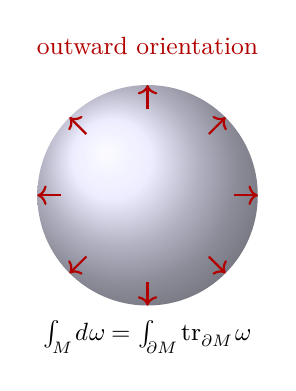
\begin{tikzpicture}[scale=1.0]
\shade[ball color=blue!12,opacity=0.8] (0,0) circle (1.4);
\foreach \a in {0,45,90,135,180,225,270,315}{
\draw[->,red!70!black,thick] ({1.1*cos(\a)},{1.1*sin(\a)})--({1.4*cos(\a)},{1.4*sin(\a)});
}
\node[red!70!black] at (0,1.9) {\small outward orientation};
\node at (0,-1.8) {\small $\int_M d\omega=\int_{\partial M}\operatorname{tr}_{\partial M}\omega$};
\end{tikzpicture}
\end{center}
\end{frame}

\begin{frame}{Summary: Stokes–Cartan in all Dim.}
\vspace{-0.3cm}
\begin{block}{Unified Framework}
For any compact oriented smooth $D$–manifold $M$ with boundary $\partial M$:
\vspace{-0.2cm}
\[
\boxed{\int_M d\omega=\int_{\partial M}\operatorname{tr}_{\partial M}\omega.}
\]
All classical theorems follow as special cases:
\vspace{-0.2cm}
\small
\begin{center}
\renewcommand{\arraystretch}{1.3}
\begin{tabular}{c|c|c}
\textbf{Dim.} & \textbf{Differential Form} & \textbf{Result}\\
\hline
$1$ & $df$ & Newton–Leibniz theorem\\
$2$ & $df$ on $\gamma$ & Gradient theorem\\
$2$ & $d(P\,dx+Q\,dy)$ & Green’s theorem\\
$3$ & $d(A\,dx+B\,dy+C\,dz)$ & Kelvin–Stokes theorem\\
$3$ & $d(P\,dy\wedge dz+Q\,dz\wedge dx+R\,dx\wedge dy)$ & Gauss divergence theorem
\end{tabular}
\end{center}
\end{block}
\end{frame}



\begin{frame}{Part I: Lecture Summary}
\begin{block}{Summary}
\begin{itemize}
\item The exterior derivative \(d_p:\Omega^pM\to\Omega^{p+1}M\) generalizes grad, curl, and divergence.
\item In \(\mathbb{R}^2\): \(d_0\) = grad, \(d_1\) = scalar curl; in \(\mathbb{R}^3\): \(d_0\) = grad, \(d_1\) = curl, \(d_2\) = div.
\item Pullback \(f^*\) transfers forms from \(N\) to \(M\) compatibly: \(d\circ f^*=f^*\circ d\).
\item Trace \(\operatorname{tr}_N=\iota_N^*\) restricts forms to submanifolds or boundaries.
\item These constructions make differential forms coordinate-independent tools for calculus on manifolds.
\end{itemize}
\end{block}
\end{frame}

\begin{frame}{Part II: Lecture Summary}
\begin{block}{Summary}
\begin{itemize}
\item Orientation is given by a nonvanishing top–degree form $\omega\in\Omega^D M$.
\item Outward vector fields define induced orientation on $\partial M$ via $\omega_S=\operatorname{tr}_{\partial M}(\iota_X\omega)$.
\item Integration of differential forms generalizes classical calculus results to manifolds.
\item Stokes–Cartan theorem unifies Newton–Leibniz, Green, Kelvin–Stokes, and Gauss divergence theorems.
\item Compact oriented manifolds admit consistent integration respecting additivity and diffeomorphism invariance.
\end{itemize}
\end{block}
\end{frame}


\begin{frame}{Thanks}
  \cmcendframe
\end{frame}

\end{document}
